\section{Introduction}
Visualization of biological networks is a core technique in systems biology for representation and analysis of complex, often heterogeneous, data. Network visualization combined with quantitative graph analysis such as detection of network modules, hub or bottleneck nodes, or cross-talk between networks can lead to novel hypothesis generation or detection of relevant patterns in biomedical data~\citep{ehlersIntroductionSurveyBiological2025}. Biological networks are of particular relevance in digital drug discovery and drug target prioritization and are used in modeling disease pathobiology as well as drug mechanism of action on a molecular level. Biological networks also represent an intuitive way of communicating and sharing research findings with collaborators or disseminating them to the broader scientific community.

Cytoscape~\citep{shannonCytoscapeSoftwareEnvironment2003} and Gephi~\citep{bastianGephiOpenSource2009} are considered gold standards for interactive network visualization with an exhaustive plugin ecosystem and rich layout capabilities, but are desktop-focused and lack portability or modern web-app features. Other tools such as STRING~\citep{szklarczykSTRINGDatabase20252025}, OmicsNet 2.0~\citep{zhouOmicsNet20Webbased2022}, NetworkAnalyst 3.0~\citep{zhouNetworkAnalyst30Visual2019} and GeneMANIA~\citep{franzGeneMANIAUpdate20182018} prioritize data integration, enrichment analysis, gene expression meta-analysis or gene function prediction, and access to extensive biological databases over visualization and customization, integrating the network viewer as a helper and not as the focus of the application. Several web-based alternatives have emerged to enhance portability. Cytoscape Web~\citep{onoCytoscapeWebBringing2025} extends the Cytoscape ecosystem with collaborative workflows for network visualization, though focusing on core functionalities with basic filtering and styling. Gephi Lite~\citep{jacomyGephiGephilite2025} shares the same graphical engine as GLL, sigma.js (\url{https://www.sigmajs.org/}), demonstrating its viability for performant browser-based exploration. However, Gephi Lite does not employ a query language and relies on graphical controls and user-written JavaScript functions for filtering. Retina~\citep{ouestwareRetina} is also based on sigma.js and allows loading GEXF files to render and share a network via links without a server where users can filter nodes by attribute, however customization capabilities are limited and the layout is fixed by the uploaded file. Graphia~\citep{freemanGraphiaPlatformGraphbased2022} provides both a desktop and web client with a powerful 2D/3D rendering engine, but focuses less on user-friendly styling, highlighting, grouping and filtering, prioritizing efficiency, enrichment, and layout, and Arena3Dweb~\citep{karatzasArena3DwebInteractive3D2021} focuses on 3D visualizations of multilayered networks.

Further noteworthy mentions of repositories and libraries complement GLL, rather than competing. NDEx~\citep{prattNDExNetworkData2015} is a framework for storing, sharing, and manipulating biological networks in the CX2 format that GLL opens and exports. Cytoscape.js~\citep{franzCytoscapejsGraphTheory2016,franzCytoscapejs2023Update2023}, together with sigma.js, are libraries for visualization and analysis to be embedded into web applications, but require programming without ready to use frontends.

We have developed Graph Lens Lite (GLL) to address the need for a browser-based tool that combines visualization power with an intuitive, streamlined interface, enabling researchers to rapidly explore and evaluate complex networks without requiring expertise in specialized software. GLL offers an expressive query language alongside graphical user interface (GUI)-based filtering, visual grouping, and fine-grained styling controls. Users can compute network metrics, apply customizable layouts, and map data attributes to visual scales. GLL exports networks as portable JSON files that capture the full application state for seamless collaboration, or as data tables for downstream analysis.

To our knowledge, none of the tools above combines the following functionalities: (i) zero-install portability as one self-contained HTML file and portable models that store the complete application state as one JSON file; (ii) a validated query language as the foundation for GUI filters, the query editor, and the AI assistant to reproduce exact filtering configurations; and (iii) schema-constrained query generation using a local language model, limited to referencing properties that exist in the network data.

\section{Materials and methods}

\subsection{Implementation and architecture}
We developed GLL using vanilla JavaScript with no front-end framework, bundled with esbuild (\url{https://esbuild.github.io}). For graph rendering and interaction, GLL uses sigma.js (\url{https://www.sigmajs.org/}), a WebGL-based rendering engine, with graphology (\url{https://graphology.github.io/}) as the underlying graph data model and for layout and metric computation, complemented by @antv/layout (\url{https://github.com/antvis/layout}) for radial, hierarchical, and concentric layouts, and by bubblesets-js (\url{https://github.com/upsetjs/bubblesets-js}) for bubble-set outlines. Custom WebGL shader modules extend the renderer with animated edge flows and a node-density heatmap layer. Spreadsheet import and export of node and edge tables use ExcelJS (\url{https://github.com/exceljs/exceljs}). The graph assistant renders Markdown responses with marked (\url{https://marked.js.org/}) and sanitizes the resulting HTML via whitelist approach using DOMPurify (\url{https://github.com/cure53/DOMPurify}). An in-memory cache store holds shared module states and the workspace data (coordinates, filters, styles, group memberships, active query and the syntax tree, and view states), which can be serialized to JSON for export, enabling session restoration.

While the core application requires no internet access, four optional network paths exist: the STRING demo loader sends requests to fetch example data. The graph assistant communicates with the configured Ollama endpoint and includes graph snapshots. The Neo4j connector queries and retrieves data from a user-specified server. And the GLL background service accepts graph network data from external applications and streams to a connected browser.

\subsection{Query language}
The query language is a purpose-built domain-specific language (DSL) that drives both filtering and selection and is based on logical combinations of conditions on node and edge properties. Each clause pairs a property path (``Section::Group::Property'') with a numeric range (``BETWEEN x AND y''), an inverted range (``LOWER THAN x OR GREATER THAN y''), categorical membership (``IN [a,b]''), or a predicate (``IS TRUE'', ``IS FALSE'', ``IS MISSING''). Parenthesized clauses are combined with the connectors ``AND'', ``OR'', and ``NOT'', where ``NOT'' is binary (``A NOT B'' means ``A AND NOT B''). The full grammar is given in the Supplementary Data. Nesting groups to any depth is supported, and the connectors are evaluated from left to right without any order of precedence, so parentheses determine the grouping. The editor renders each token as spans with dedicated CSS classes for syntax highlighting, validates on each change and flags empty clauses, missing connectors, unmatched brackets, unrecognized tokens or invalid property paths. Valid queries are decoded as a nested syntax tree that is used to evaluate each element in the graph.

\subsection{Graph assistant}
The graph assistant's system prompt encodes GLL's main functionalities and instructs the model to reference UI controls using predefined glyphs that are rendered as clickable action buttons in its replies, and to request a query when the user asks to filter the graph. Query generation is split into two phases. In the first, on recognizing that a query is needed, the model appends a block (``<<<QUERY\_INTENT>>>{summary, scope}<<<END>>>'') to its reply, which is stripped from the displayed response. In the second phase, a separate structured-output call (temperature 0) sends a JSON schema to the model using Ollama's ``format'' parameter. The schema allows only the graph's existing property paths as fields and only the query language's operators. The model therefore cannot emit a non-existent property or an unsupported operator. The generated structured output is rendered to a query string that is then decoded and evaluated in the same manner as typed or GUI-built queries. If the structured output fails to render to a valid query (e.g. an empty membership list), a single repair pass retries, remapping any invalid property to its nearest valid path by Levenshtein distance.

\subsection{Packaging and distribution}
% TODO: update at release 1.18.0 freeze (I will do it)
GLL is released under the MIT license. Desktop builds for Windows, macOS, and Linux are produced with electron-builder (\url{https://www.electron.build/}) on Electron 43 (\url{https://www.electronjs.org/}). A platform-independent single-file build is produced with inline-source (\url{https://github.com/popeindustries/inline-source}), which inlines the application bundle, stylesheets, and assets into one self-contained HTML file of about 2.7 MB that runs in any modern browser. Releases are versioned semantically and distributed through GitHub Releases and GitHub Pages, with a live demo at  \url{https://delta4ai.github.io/GraphLensLite/}. GLL can also run as a background service built with Node.js (\url{https://www.nodejs.org}) that exposes a token-protected REST endpoint, accepting data in GLL's JSON format and streaming it to connected browsers over Server-Sent Events, so external applications can hand off network data to GLL for interactive exploration, with concurrent users kept separate through named sessions, without writing intermediate files. A Dockerfile builds the viewer and the background service into one container image that runs with Docker or Podman. The codebase is covered by over 2,400 automated tests across 153 files, written with Vitest (\url{https://vitest.dev/}).

\section{Results}

% TODO: update screenshot, adapt references (I will do it)
\begin{figure*}[!t]
    \centering
    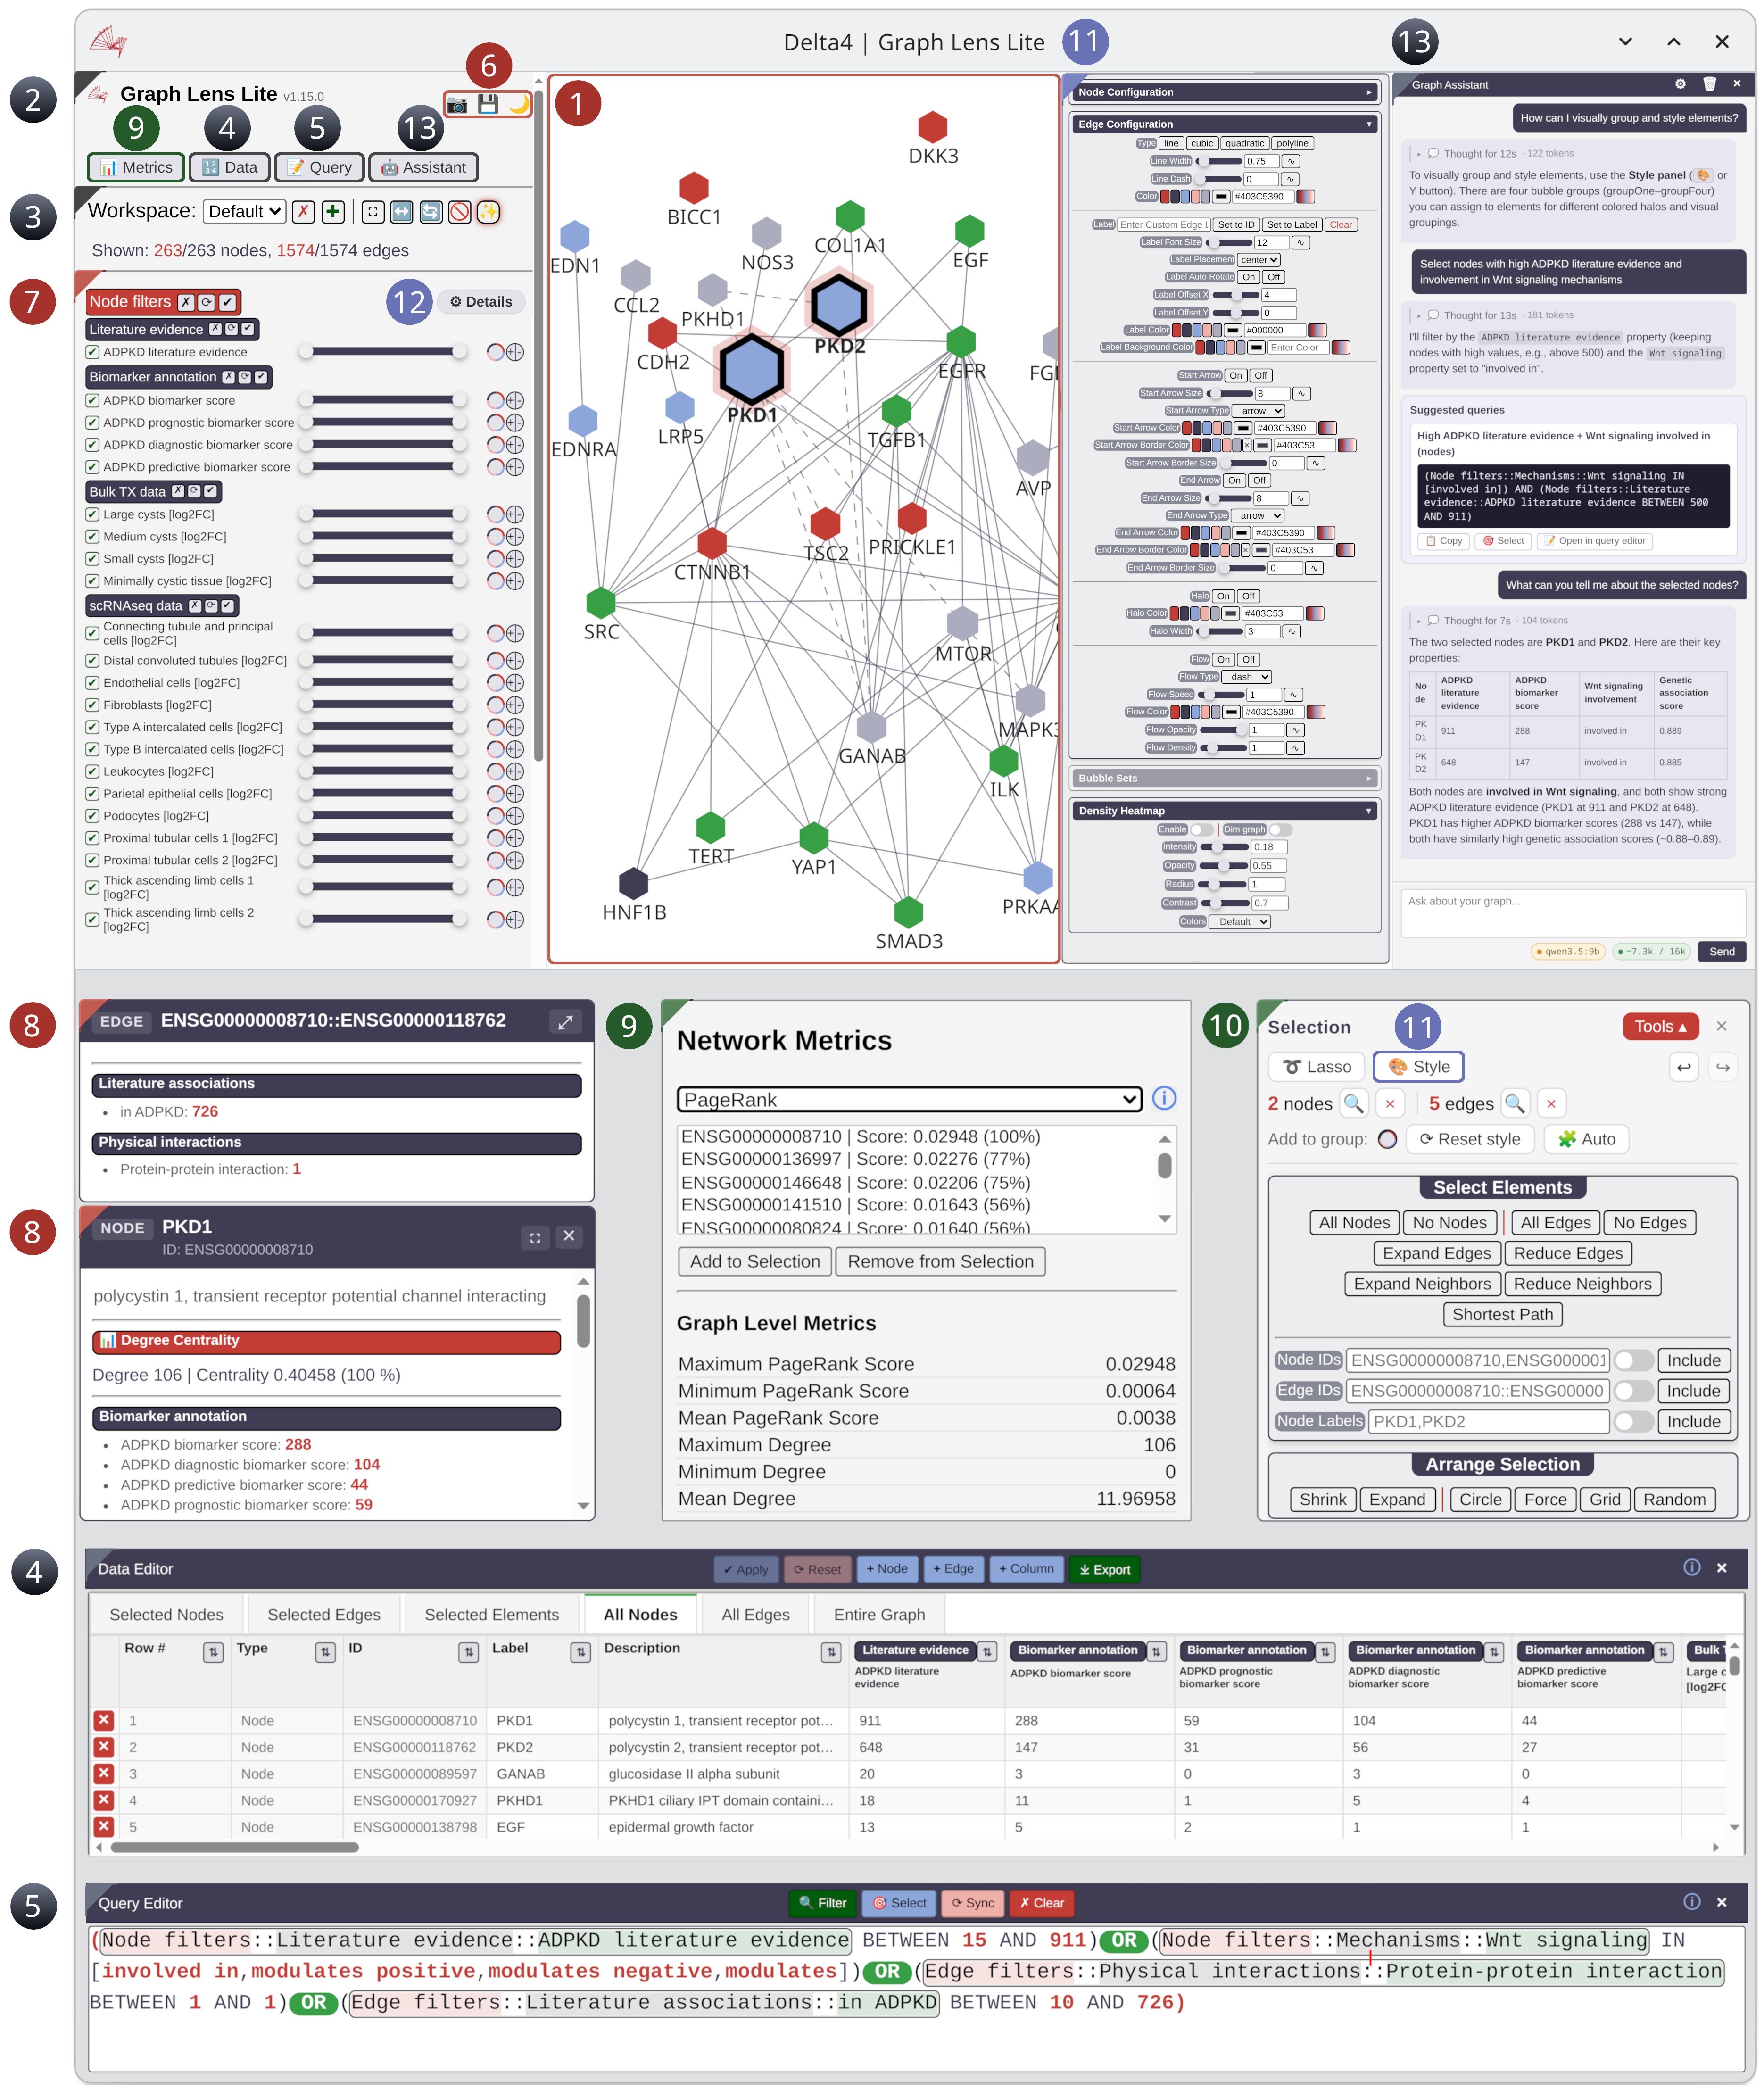
\includegraphics[width=\textwidth,height=\textheight,keepaspectratio]{main-figure.png}
    \caption{The graphical user interface of Graph Lens Lite. (1) Main network view, (2) File import, (3) Workspace management, (4) Data editor, (5) Query editor, (6) Network and image export, (7) Node and edge filtering, (8) Node and edge tooltips, (9) Network metrics, (10) Selection panel, (11) Style panel, (12) Edit mode, (13) Graph assistant.}
    \label{fig:main-figure}
\end{figure*}

GLL presents network exploration through a single-page interface built around a central network view and a set of dedicated panels for data input, filtering, selection, styling, metrics, data and query editors, and an assistant (Figure~\ref{fig:main-figure}).

\subsection{Data input}
GLL accepts spreadsheets containing node and edge tables, a JSON format preserving the application state, or GraphML and CX2 network file formats. Input data require an ``ID'' column for nodes and ``Source ID/Target ID'' columns for edges. Optional columns may specify visual attributes such as labels, shapes, sizes, colors, or coordinates. Custom properties containing user data can be added as new columns, with optional group labels in square brackets. A template with column specifications, example values, and supported data types is available on GitHub and can also be generated from within the application. Additionally, a demo loader enables direct fetching of protein--protein interaction networks from the STRING~\citep{szklarczykSTRINGDatabase20252025} database.

Data can be queried from a Neo4j graph database (\url{https://neo4j.com/}) via Cypher statements with a check beforehand how much data will be retrieved and options to exclude selected properties before rendering. A running GLL service instance can furthermore be used to send network data from external applications and serve visualizations back to the user's browser without manual file handling (see packaging and distribution).

\subsection{Guided tour}
On application launch, users can start an interactive guided tour that loads a small example protein network and walks the user step-by-step through the application's core components. At each step the tour highlights relevant icons, opens panels, and explains the usage with live interface components, lowering the entry barrier for new users.

\subsection{Graphical user interface}
The numbered elements in Figure~\ref{fig:main-figure} correspond to the following components:

\noindent
\textbf{(1) Main network view:} The central window for displaying and interactively exploring the loaded network through panning, zooming, node dragging, hovering over elements to highlight adjacent elements, and an overview minimap. \\
\textbf{(2) File import:} Open the launch screen to load network data from spreadsheets (node and edge tables) or portable GLL JSON files, fetch protein--protein interaction data from the STRING database, or query a Neo4j database. \\
\textbf{(3) Workspace management:} Create and switch between independent workspaces, each preserving its own layout, filters, queries, groupings, and styles. Reset the layout, fit the graph to view, hide disconnected nodes, or toggle highlight effects. \\
\textbf{(4) Data editor:} Spreadsheet-style interactive table for adding, deleting, and editing nodes, edges, and their properties, defining new custom property columns, and export the entire network, nodes, edges, or filtered sub-networks. \\
\textbf{(5) Query editor:} Editor for nested graph filtering and selection using a custom query language, supporting Boolean connectors, numeric range, categorical membership, and Boolean and missing-value predicates. Synchronizes with the GUI filtering panel. \\
\textbf{(6) Network and image export:} Save the complete application state to a portable GLL JSON file for session restoration and sharing, or export the current view as high-resolution PNG or vector SVG. \\
\textbf{(7) Node and edge filtering:} GUI-based selection and visual grouping, filtering via range sliders for numeric properties and category checklists for categorical values, synchronized with the query language. \\
\textbf{(8) Node and edge tooltips:} Displays metadata for the selected node or edge element on click. \\
\textbf{(9) Network metrics:} Compute topological centrality measures (degree, betweenness, closeness, eigenvector, and PageRank) to rank, filter, and select graph elements, with graph-level statistics and illustrative documentation for each method. \\
\textbf{(10) Selection panel:} Shows current node and edge selection counts with lasso selection and undo/redo history. An expandable section provides additional focus, search, neighbor/edge expansion, shortest-path tracing between two selected nodes, and per-selection sub-layout controls. \\
\textbf{(11) Style panel:} Edit node, edge, and bubble-group styles, and map data properties or computed network metrics onto visual scales (continuous and discrete color scales, numeric size scales). \\
\textbf{(12) Edit mode:} Toggles fine-grained configuration for GUI-based filtering via precise numeric thresholds. \\
\textbf{(13) Graph assistant:} Context-aware AI assistant that answers natural-language questions about the network, translates them into runnable queries, and summarizes the current selection. \\

\subsection{Features and workflow}
GLL starts by loading network data from spreadsheet files containing node and edge tables (Figure~\ref{fig:main-figure}.2) or from JSON files. User-supplied properties (coordinates, styling options) are applied where specified. Alternatively, users can fetch demo data from the STRING database or query a Neo4j database. The workspace management panel (Figure~\ref{fig:main-figure}.3) allows switching between independent environments, each preserving its own aesthetics, layouts, filters, and queries.

Once loaded, users can explore the network structure through multiple approaches. The selection panel (Figure~\ref{fig:main-figure}.10) enables element search, selection, expansion to connected neighbors, and tracing the shortest path between two selected nodes on the currently visible network. Metadata for selected node and edge elements appear in specific tooltips (Figure~\ref{fig:main-figure}.8). For deeper analysis, GLL computes five node-centrality measures (degree~\citep{freemanCentralitySocialNetworks1978}, betweenness~\citep{freemanSetMeasuresCentrality1977a}, closeness~\citep{bavelasCommunicationPatternsTaskOriented1950a}, eigenvector~\citep{bonacichFactoringWeightingApproaches1972,newmanMathematicsNetworks2018a} and PageRank~\citep{brinAnatomyLargescaleHypertextual1998a}) together with graph-level statistics including network density and centralization, to identify key nodes (Figure~\ref{fig:main-figure}.9). Users can select a metric and examine one or more highly ranked nodes, with graph-level statistics displayed in the metric panel. In-app documentation describes each metric's methodology and provides references to relevant literature. The network can be arranged with a range of layout algorithms: live-animating force-directed (ForceAtlas2~\citep{jacomyForceAtlas2ContinuousGraph2014}), hierarchical, circular, radial, concentric, and circle-packing, applied either to a selection or across the entire workspace, with animated transitions between layouts and an optional overlap-removal pass.

GLL supports network filtering through graphical controls (Figure~\ref{fig:main-figure}.7), an edit mode for precise numeric input (Figure~\ref{fig:main-figure}.12), and a query editor for complex, nested operations (Figure~\ref{fig:main-figure}.5). All interfaces are synchronized, acting on the same underlying node and edge properties. The query language (see Materials and methods) is validated as the user types against the loaded graph's property hierarchy, and a single query drives both filtering and selection while staying consistent with the GUI controls. Contextual help is accessible via an adjacent icon.

GLL integrates an optional, context-aware AI assistant designed for a locally hosted model (Figure~\ref{fig:main-figure}.13), lowering the barrier to exploration by translating questions into instructions, queries and summaries. Each request embeds a snapshot of the current workspace, including node and edge counts, the property hierarchy with data types, active filters, the current query, and the currently selected nodes and edges including their property values and computed network metrics. Responses are grounded in the live graph state. When asked for a query, the assistant constructs a schema-constrained structured query representation based on the loaded graph's properties. The query is constrained to the data, referencing only real properties and supported operators. Results can be applied to select elements via rendered action buttons, or loaded into the query editor for further refinements.

The assistant communicates with an Ollama server and is configurable in the panel's settings menu. By using a local endpoint, graph data stays within the user's machine or network. Non-local hosts trigger warnings and indicate that messages include a snapshot of the graph data and are transferred to that host. Enabling the assistant therefore requires a running Ollama instance and any downloaded instruction-following model capable of reliably creating structured JSON output. Response quality depends on the chosen model.
On a benchmark of 52 questions about the case-study network and an airport network (Supplementary Table S2), the query generated by \texttt{qwen3.5:9b}~\citep{qwen3.5} selected exactly the same elements as a hand-written reference query for 88.5\,\% of the questions, including declining every question the data could not answer, with a median response time of 25\,s on a workstation graphics processing unit (GPU) with 16\,GB of memory. The smaller \texttt{qwen3.5:4b} reached 75.6\,\% and the three other models tested 51.9 to 75.0\,\%; the weakest of them never declined an unanswerable question and returned a query on an unrelated property instead. Running a local endpoint prevents transmission of potentially sensitive network data to third-party services. A context-budget indicator reports how much of the selected model's context window the next request will consume and warns users when a request would exceed the threshold and be truncated.

The styling panel (Figure~\ref{fig:main-figure}.11) offers extensive visual customization options for nodes, edges, and groups. Properties such as geometry (shape, size), color (fill, border, line), labels (text, placement, font), and annotations (badges, halos, arrows) can be configured independently for each element type. Edges can additionally render animated directional flow, with selectable flow styles (e.g. comet or chevron), adjustable opacity and density, to express directionality or magnitude. A node-density heatmap can be drawn to highlight dense regions of the layout, with controls for intensity, opacity, radius, contrast, thresholds, and predefined color maps. Up to four bubble sets~\citep{collinsBubbleSetsRevealing2009} allow visual grouping of nodes with adjustable appearance, populated manually or automatically through Louvain community detection~\citep{blondelFastUnfoldingCommunities2008}. Numeric and categorical attributes, whether user-supplied or computed from network metrics, can be dynamically mapped to visual features like color and size to highlight importance. Nodes can be rendered as pie charts that encode several numeric or categorical properties as wedges, adding a data dimension beyond color and size.

GLL includes an integrated data editor (Figure~\ref{fig:main-figure}.4) for modifying network data in tabular format. Supported operations include column sorting, cell editing, node and edge addition or deletion, table reset, and export to spreadsheet format. Users can also add new columns to define custom properties for nodes or edges, which become immediately available in the filtering and styling interfaces, enabling graph creation and manipulation entirely within the application.

A graph can be exported in GLL's native JSON format, as GraphML or CX2 for other network tools, or as a high-resolution PNG or vector SVG image (Figure~\ref{fig:main-figure}.6). JSON exports preserve the complete application state, including views, filters, coordinates, and styling, enabling session restoration and collaborative sharing.

\subsection{Modeling autosomal dominant polycystic kidney disease}
In this case study, we use GLL to visualize the molecular pathobiology of autosomal dominant polycystic kidney disease (ADPKD), two drugs, and the interference signatures that link each drug to the disease network. The corresponding dataset is provided as an Excel file in GLL's import format (Supplementary datafile S1; \url{https://github.com/Delta4AI/GraphLensLite/tree/main/manuscript}) so readers can reproduce these views and explore the tool's features interactively.

\begin{figure}[!t]
    \centering
    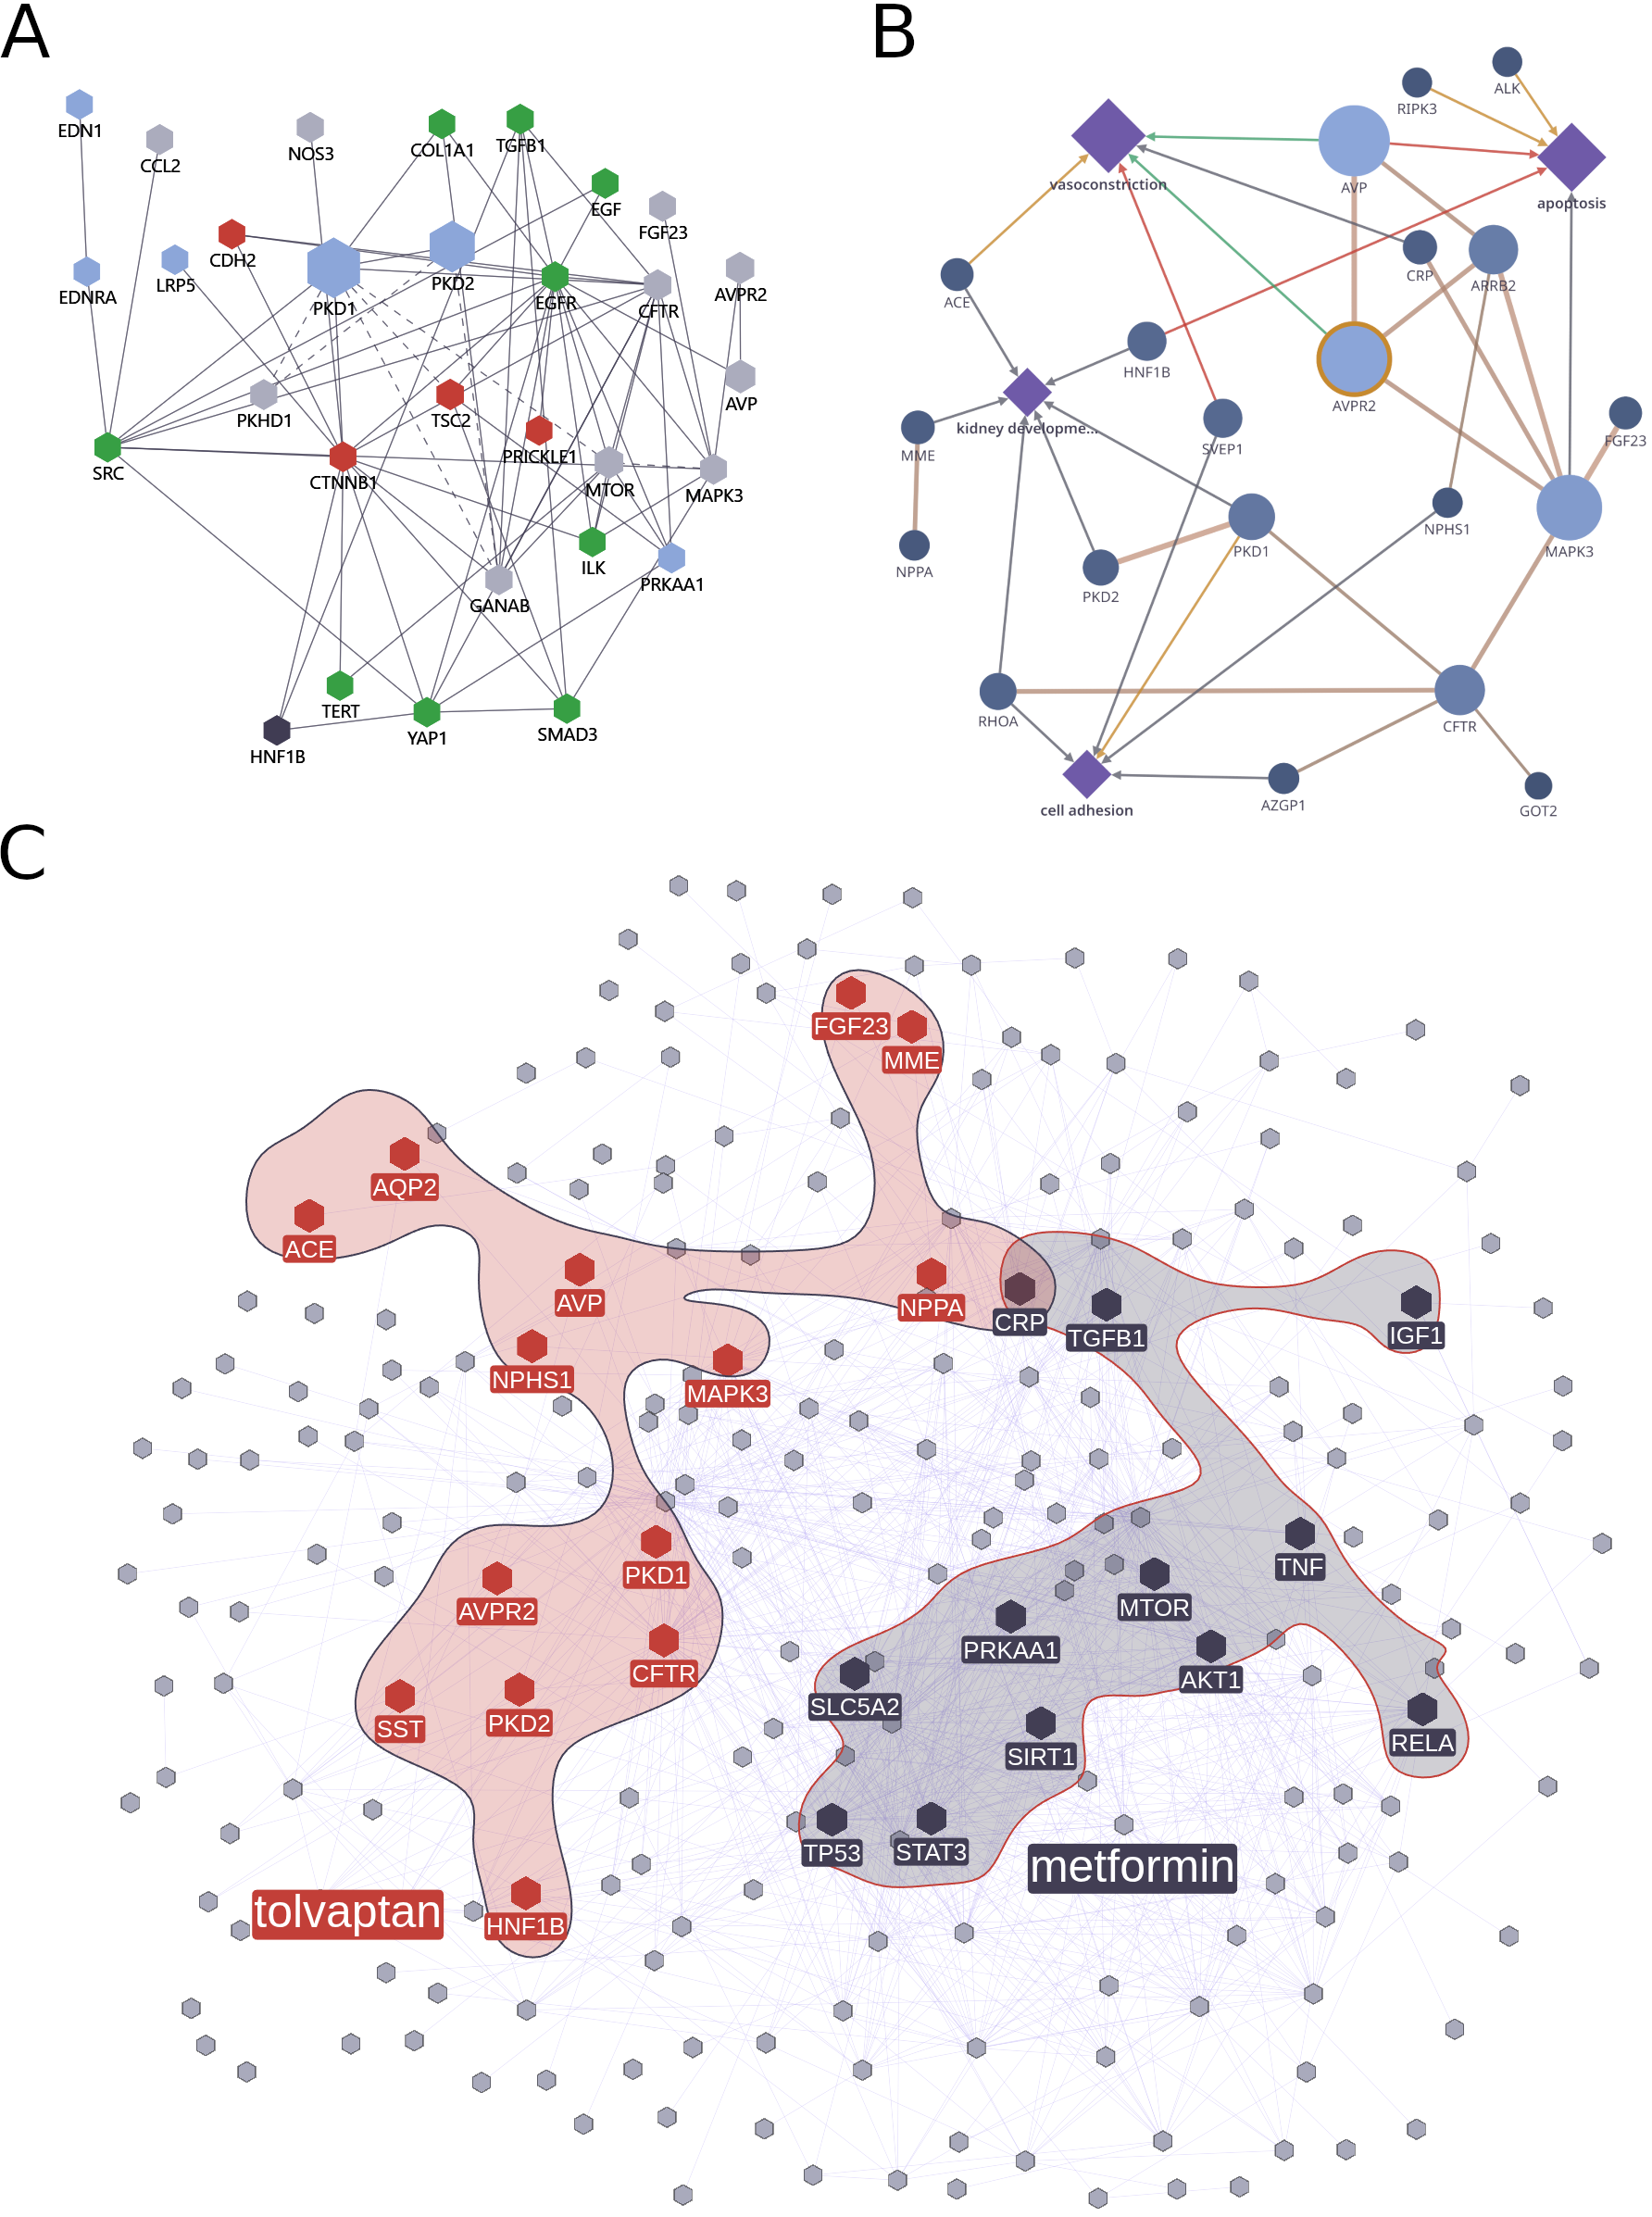
\includegraphics[width=\columnwidth,keepaspectratio]{adpkd-figure.png}
    % TODO(figure): Panel A encodes positive/negative modulation in green/red,
    % which is not colour-blind safe; re-export with a colour-blind-safe
    % palette (e.g. blue/orange) and update the caption and the Results text.

    \caption{Visualizing disease and drug models. Panel A: Proteins of the ADPKD molecular model being associated with the Wnt signaling pathway (in green for positive modulation of the pathway, red for negative modulation of the pathway, dark blue for modulation of the pathway, and light blue for genes being pathway members without any further information on regulation) as well as additional molecules being associated with ADPKD that are linked to members of the Wnt signaling pathway (in gray) via either protein--protein interactions (solid edges) or literature co-annotations in the context of ADPKD (dashed edges). Panel B: The drug MoA molecular model for tolvaptan showing key associated proteins (circles) as well as associated molecular mechanisms (purple diamonds). Node size and shade scale with a composite evidence score summed over the protein interactions, mechanism assignments, and gene--drug co-annotations of each node; the gold ring marks the direct drug target AVPR2. Tan edges are protein--protein interactions from OmicsNet, with width scaling with interaction weight. Arrows link proteins to mechanisms and are colored by the annotated effect (green, positive; red, negative; gold, modulating; gray, not specified). Panel C: The largest connected component of the ADPKD molecular model with the interference signatures for tolvaptan (red) and metformin (dark slate) drawn as bubble sets. The two drug signatures share one node, CRP.}
    \label{fig:adpkd-model}
\end{figure}

ADPKD is the most common inherited kidney disorder, characterized by the gradual development and enlargement of multiple cysts in both kidneys, which ultimately leads to a progressive deterioration in kidney function~\citep{formicaMolecularPathwaysInvolved2020}. ADPKD is a multi-factorial disease involving different disease mechanisms and molecular pathways. The exact mechanisms of ADPKD development and progression are still not fully understood and a better understanding of disease pathobiology is the basis for the discovery of novel drug targets and the development of new treatment options.
This paper introduces a new molecular model of ADPKD pathobiology, which we built by consolidating a set of biomedical data on ADPKD and explored using GLL.
% NOTE(authors, 2026-11-04): construction details of the Hyper-C literature
% co-annotations are not given here; they are available to reviewers on request.
Literature associated ADPKD molecular features (genes and proteins) were extracted from Delta4's Hyper-C software platform that consists of sentence-level literature co-annotations between individual molecular features and ADPKD. This set of literature-associated ADPKD molecular features was complemented by genes showing differential expression in ADPKD as compared to healthy tissue based on Omics data.
We downloaded the ADPKD microarray dataset with the accession number GSE7869 (Affymetrix Human Genome U133 Plus 2.0, GPL570) from the Gene Expression Omnibus and re-analyzed the dataset to generate lists of differentially expressed genes. In the original study~\citep{songSystemsBiologyAutosomal2009}, global gene expression profiling was conducted on renal cysts of different volumes, and non-cancerous renal cortical tissue from nephrectomized kidneys was used as controls; of the 21 samples, only three are normal cortex controls, which limits the statistical power of each comparison. Differential gene expression analysis involved data normalization, statistical modeling using linear models, identification of regulated genes based on $\log_2$ fold-change ($\log_2 \text{FC}$) and adjusted p-values. Ultimately, the ADPKD phenotype model was enriched with 20 genes which showed absolute $\log_2 \text{FC}$ > 2 and adjusted p-values < 0.05 across all four comparisons (large, medium, and small cysts, as well as minimally cystic tissue as compared to healthy tissue from nephrectomized kidneys respectively). In addition, we re-analyzed a single-nucleus RNA sequencing (sn-RNA-Seq) dataset with the GEO accession number GSE185948, offering insights into the cellular heterogeneity of ADPKD~\citep{mutoDefiningCellularComplexity2022}. Genes with a p-value < 0.05 were included as candidates in the analysis.
% TODO(authors): snRNA-seq threshold is an unadjusted p < 0.05 -- was an
% FDR/adjusted p-value used? If so, state the method; if not, say
% "unadjusted" explicitly and justify (GSE7869 above uses adjusted p-values).

Ultimately, the ADPKD phenotype molecular model was enriched with genes that were expressed in at least one cell type with absolute $\log_2 \text{FC}$ values > 2.5. In addition we retrieved information on genetic associations with ADPKD from the OpenTargets platform~\citep{bunielloOpenTargetsPlatform2025}. Expression in healthy tissue and relevant renal cell types of molecular features of the ADPKD molecular model, quantified as normalized transcripts per million (nTPMs), were extracted from the Human Protein Atlas consensus expression profile dataset~\citep{karlssonSingleCellType2021}. Information on subcellular location for features of the ADPKD molecular model was retrieved from UniProt~\citep{ahmadUniProtWebsiteAPI2025}. Finally, we assigned molecular features of the ADPKD molecular model to mechanisms being discussed in recent reviews to be associated with ADPKD disease development and progression. Assignment of molecular features to mechanisms was done using the Gene Ontology (GO) annotation.

The resulting novel ADPKD molecular model consists of 263 molecular features connected by 1,574 edges (Supplementary datafile S1). Edges in the constructed network consist of protein--protein interactions consolidated from IntAct~\citep{orchardMIntActProjectIntAct2014} and BioGRID~\citep{oughtredBioGRIDDatabaseComprehensive2021}, interactions inferred from co-membership in Reactome complexes~\citep{ragueneauReactomeKnowledgebase20262026}, as well as of literature sentence-level co-annotations of publications focusing on ADPKD using the catalogs of molecular features and phenotypes as given in Delta4's Hyper-C software platform.

The constructed molecular model can now be used to explore the pathobiology of ADPKD by either filtering for (i) certain molecular mechanisms, (ii) individual cell types, (iii) the most up- or down-regulated genes in renal tissue or specific cell types, (iv) the most central genes based on graph properties like node degree or betweenness among others. Figure~\ref{fig:adpkd-model}A for example shows genes of the Wnt signaling pathway (in green for positive modulation of the pathway, red for negative modulation of the pathway, dark blue for modulation of the pathway, and light blue for genes being pathway members without any further information on regulation) as well as additional molecules being associated with ADPKD that are linked to members of the Wnt signaling pathway (in gray) via either protein--protein interactions or co-annotations in the context of ADPKD. This network view allows investigating novel connections of Wnt signaling pathway members with ADPKD-associated proteins.

The molecular model can subsequently be used to (i) screen for compounds showing beneficial impact on dysregulated disease mechanisms as shown previously in other renal diseases~\citep{gebeshuberComputationalDrugRepositioning2023}, (ii) identify drug targets of interest, investigate cell-cell interaction analysis to identify relevant receptor-ligand pairs following previously reported analyses~\citep{evgeniouMetaAnalysisHumanTranscriptomics2021}, or (iii) prioritize drug targets for the development of new chemical entities.

The only FDA-approved treatment for ADPKD is the selective vasopressin V2-receptor (AVPR2) antagonist tolvaptan. We generated a molecular mechanism of action model for tolvaptan based on literature associated tolvaptan molecular features (genes and proteins) (Figure~\ref{fig:adpkd-model}B). Molecular features were extracted from Delta4's Hyper-C software platform that consists of sentence-level literature co-annotations between individual molecular features and tolvaptan. Mechanisms were assigned to molecular features via GO annotation. The constructed MoA molecular model can subsequently be used to assess drug mechanism of action on disease pathobiology via network interference analysis~\citep{heerspinkCanagliflozinReducesInflammation2019,gebeshuberComputationalDrugRepositioning2023,evgeniouIntegrativeAnalysisDrug2025} with interfering nodes between the ADPKD molecular model and the tolvaptan drug MoA molecular model making up the interference signature. We can subsequently also evaluate and graphically display how two different drugs interfere with disease pathobiology on the molecular level.

Figure~\ref{fig:adpkd-model}C displays the interference signatures of tolvaptan (in red) and metformin (in dark slate), a compound currently being tested in the ongoing phase 3 IMPEDE-PKD trial (NCT04939935) and being discussed as a compound to be combined with tolvaptan to treat patients with ADPKD~\citep{stanleySecondaryAnalysisConcurrent2024}. The two drug signatures, covering 15 (tolvaptan) and 12 (metformin) of the 263 nodes in the network, are largely distinct and share only CRP. The supplementary datafile S1 highlights the drug signatures as separate columns to allow reproduction of Figure~\ref{fig:adpkd-model}C. The network visualization shows at a glance which regions of the ADPKD model are affected by each of the drugs, serving as a starting point for hypothesis generation on drug combinations.

% ───────────────────────────────────────────────────────────────────────────
\section{Discussion}
We have developed GLL, an interactive, browser-based network viewer for exploring and sharing biological networks through a streamlined interface. It combines an expressive query language with topological network analysis, interactive filtering, visual grouping, customizable layouts, a data editor, fine-grained property-based styling, animated edge-flow visualization, community detection, and a context-aware, locally hosted AI assistant, supporting the visual exploration of molecular models of disease pathobiology or drug mechanism of action. GLL requires only a web browser for core functionality: it is distributed as a single self-contained HTML file, which can be combined with a network model into a compact archive of under 3 MB for sharing, while platform-specific Electron bundles provide native desktop applications across Windows, macOS, and Linux. This minimal footprint enables collaboration, long-term stability, and offline operation.

Table~\ref{tab:tools} compares GLL against biomedical network exploration tools across their deployment surface (web, desktop, or single-file HTML), offline usability versus server dependency, portability of the exploration state, editability of the underlying data, the presence of a query language for complex filtering, and the availability of an AI assistant.

\begin{table}[!htbp]
\centering
\caption{Comparison of selected network analysis and visualization tools for biomedical research. \emph{Single-file HTML}: the entire application is one HTML file that runs locally with no install procedure or server. \emph{Offline-ready}: core functionality works without an external server or third-party API (optional demo data loaders may still require network access). \emph{Portable state}: the complete application state (data, view, filters, layout, and styling) exports and re-imports as a single file. \emph{Data editor}: nodes, edges, and custom properties can be created, edited, and deleted from the GUI. \emph{Query DSL}: a domain-specific query language for complex graph filtering is available. \emph{AI assistant}: built-in assistant powered by a locally hosted open-source model for natural-language interaction. Cells: \checkmark{} present, \LEFTcircle{} partial (see footnote), -- absent.}
\label{tab:tools}
\footnotesize
\setlength{\tabcolsep}{3pt}
\renewcommand{\arraystretch}{1.1}
\newcommand{\rh}[1]{\rotatebox[origin=l]{90}{#1}}
\newcommand{\pt}[1]{\LEFTcircle\textsuperscript{#1}}
\begin{tabularx}{\columnwidth}{@{}X *{8}{>{\centering\arraybackslash}p{0.55cm}}@{}}
\toprule
Tool & \rh{Web} & \rh{Desktop} & \rh{Single-file HTML} & \rh{Offline-ready} & \rh{Portable state} & \rh{Data editor} & \rh{Query DSL} & \rh{AI assistant} \\
\midrule
Graph Lens Lite                                                  & \checkmark & \checkmark & \checkmark & \checkmark & \checkmark & \checkmark & \checkmark & \checkmark \\
Cytoscape~\citep{shannonCytoscapeSoftwareEnvironment2003}        & --         & \checkmark & --         & \checkmark & \checkmark & \checkmark & \pt{a}     & \pt{b}     \\
Cytoscape Web~\citep{onoCytoscapeWebBringing2025}                & \checkmark & --         & --         & --         & \checkmark & \checkmark & --         & --\textsuperscript{c} \\
Gephi~\citep{bastianGephiOpenSource2009}                         & --         & \checkmark & --         & \checkmark & \checkmark & \checkmark & --         & --         \\
Gephi Lite~\citep{jacomyGephiGephilite2025}                      & \checkmark & --         & --         & \checkmark & \checkmark & \checkmark & --\textsuperscript{d} & -- \\
Graphia~\citep{freemanGraphiaPlatformGraphbased2022}             & \checkmark & \checkmark & --         & \checkmark & \checkmark & \pt{e}     & --\textsuperscript{f} & -- \\
OmicsNet 2.0~\citep{zhouOmicsNet20Webbased2022}                  & \checkmark & --         & --         & --         & \pt{g}     & --         & --         & --         \\
STRING~\citep{szklarczykSTRINGDatabase20252025}                  & \checkmark & --         & --         & --         & \pt{h}     & --         & --         & --\textsuperscript{i} \\
Reactome~\citep{ragueneauReactomeKnowledgebase20262026}          & \checkmark & --         & --         & --         & \pt{h}     & --         & --         & --\textsuperscript{i} \\
  \bottomrule
\addlinespace[2pt]
\multicolumn{9}{@{}p{\columnwidth}@{}}{\scriptsize
	\textsuperscript{a}Cytoscape offers Lucene full-text search and a GUI filter builder, but no unified query language.\quad
	\textsuperscript{b}CyChat, a Cytoscape desktop app (Cytoscape App Store), adds a chat assistant, including local Ollama models~\citep{lieboldCyChatConversationalCytoscape2026}; it is an add-on, not built in.\quad
	\textsuperscript{c}Cytoscape Web's LLM Query interprets gene sets through ChatGPT (user-supplied OpenAI API key); no local model.\quad
	\textsuperscript{d}Gephi Lite filters through graphical controls and user-written JavaScript functions, not a query language.\quad
	\textsuperscript{e}Graphia allows editing attributes and deleting nodes, but not creating them.\quad
	\textsuperscript{f}Graphia's transform GUI is backed by a DSL internally but is not user-queryable.\quad
	\textsuperscript{g}OmicsNet 2.0 offers JSON export, but re-import was unreliable in our testing.\quad
	\textsuperscript{h}STRING and the Reactome Pathway Browser encode a shareable state in a URL, not a full workspace.\quad
	\textsuperscript{i}STRING Chat (built on STRING's MCP server) and Reactome's React-to-Me are cloud services.\quad}
\end{tabularx}
\end{table}

While Table~\ref{tab:tools} provides a direct comparison across tools, some entries require further explanation to highlight GLL's distinct capabilities. STRING Search~\citep{szklarczykSTRINGDatabase20252025} (\url{https://string-db.org/cgi/input}) and the Reactome Pathway Browser~\citep{ragueneauReactomeKnowledgebase20262026} (\url{https://curator.reactome.org/PathwayBrowser}) provide shareable states by encoding the current selection and analysis parameters into a URL, rather than serializing the full workspace. OmicsNet 2.0~\citep{zhouOmicsNet20Webbased2022} offers JSON export whose re-import proved unreliable in our testing, reloading as a differently styled network including more than the exported set of nodes. To elaborate on domain specific query languages integrated into the application, Graphia's~\citep{freemanGraphiaPlatformGraphbased2022} transform GUI is backed by a DSL internally but does not expose it for users to write or share, while Cytoscape~\citep{shannonCytoscapeSoftwareEnvironment2003} combines Lucene-style full-text search with a visual GUI-based filter engine, rather than a single, shareable query surface. GLL couples one validated query language with its GUI controls, so the same expression can be written by hand, constructed through the interface, or generated by the assistant.

Most recently, conversational assistants appear across the field. Cytoscape Web's LLM Query feature allows interpretation of gene sets using OpenAI's GPT models (\url{https://openai.com/}) by providing a user-supplied API key. For Cytoscape Desktop, the CyChat extension adds a chat assistant that includes local Ollama models~\citep{lieboldCyChatConversationalCytoscape2026}. STRING Chat (\url{https://string-db.org/cgi/chat}, built on STRING's MCP server) and Reactome's React-to-Me~\citep{ragueneauReactomeKnowledgebase20262026} are cloud services. GLL's assistant differentiates by generating queries with a locally hosted model and constrainted to a schema built from the loaded graph. By referencing only properties that exist, and by formulating queries that are validated by the same language that powers GUI filters and the query editor, its output can be inspected, edited and applied like hand-written queries. GLL is therefore positioned in a niche and does not replace established platforms. While it cannot compete with the plugin ecosystems of Cytoscape and Gephi~\citep{bastianGephiOpenSource2009} or the diversity and breadth of databases offered by STRING and Reactome, it complements them by providing a portable, offline-capable, and highly customizable way to explore focused, curated networks. Similar to Gephi Lite, GLL uses WebGL via sigma.js as a GPU-accelerated engine to sustain interactive exploration of large networks, and combines it with styling, filtering and grouping capabilities described above.

\subsection{Limitations}
GLL targets curated, interpretable networks rather than genome-scale topologies.
With default styling, zooming and panning stayed at or above 30 frames per second up to 50,000 nodes and 250,000 edges on a workstation GPU, and up to 25,000 to 50,000 nodes on a laptop's integrated GPU (Supplementary Table S1). Per-element styling, such as curved edges and labels on every node, lowers this limit on the workstation to 10,000 to 25,000 nodes, and the animated overlays (edge flow, groups and the density heatmap) to 1,000 to 5,000 nodes.

% TODO(freeze): re-check the feature limitations below (metric count,
% directed metrics, path tracing, formats) against the release build.
The network metric analysis covers five centrality measures computed on undirected graph data, and community structure can be revealed through Louvain community detection mapped onto visual groups. Directed-graph metrics are not yet supported. Path tracing between selected features is supported as an unweighted shortest path computed on the visible (filtered) subgraph. Weighted path costs are not considered, and only a single shortest path is returned when several of equal length exist.

GLL is compatible with GraphML and CX2 formats to exchange networks with tools such as Cytoscape, Gephi, and NDEx. These formats carry node and edge attributes, labels and positions. Styles, workspaces and groups are preserved only in GLL's JSON format.

Keeping GLL's query language and GUI synchronized proved difficult, as nested statements and negations do not map cleanly to graphical controls given the current design. The filtering panel therefore offers a single join mode applied across all clauses — OR by default or AND, the latter with an optional complete-cases mode — but cannot express the arbitrary nesting or negation supported by the raw query language. When a raw query is modified and applied to filter the graph, the GUI filtering panel is locked and flagged with a note that the query takes precedence, with the option to unlock it by resetting the query to match the GUI's state. Value changes, property selections, and the join mode remain synchronized as the query is edited, whereas nesting and negation do not.

\section{Acknowledgements}
Claude (Anthropic) was used to check the manuscript for errors in grammar and clarity and to suggest revisions, which the authors reviewed and rewrote. Software development was assisted by AI coding agents under the authors' direction; all code was reviewed and tested by the authors. The authors take full responsibility for the content of this article.

\textit{Author contributions:} M.L.: conceptualization; resources; software; visualization; writing - original draft, review \& editing. K.K.-I.: data curation; validation; writing - review \& editing. L.F.: validation; writing - review \& editing. S.M.W.: validation; writing - review \& editing. F.B.: validation; writing - review \& editing. E.B.: validation; writing - review \& editing. L.G.: validation; writing - review \& editing. P.A.: validation; writing - review \& editing. P.H.: data curation; validation; writing - review \& editing. J.L.: data curation; funding acquisition; validation; writing - review \& editing. P.P.: conceptualization; data curation; funding acquisition; supervision; validation; writing - original draft, review \& editing. K.K.: funding acquisition; supervision; validation; writing - review \& editing.

\section{Supplementary Data}
Supplementary data is available at NAR online.

\section{Conflict of interest}
K.K. is a co-founder of Delta4 GmbH (Vienna, Austria). M.L., K.K.-I., L.F., S.M.W., F.B., E.B., L.G., P.A., and P.P. are employed at Delta4 GmbH (Vienna, Austria).

\section{Funding}
This project has received funding from the Austrian Research Promotion Agency (FFG) under grant agreement number 915133 (ADPKD Drug Discovery). Enrico Bono is supported by a grant from the European Union's Horizon Europe Marie Skłodowska-Curie Actions Doctoral Networks program project PICKED (HORIZON-MSCA-2023-DN-01, grant number 101168626). Louiza Galou is supported by a grant from the European Union's Horizon Europe Marie Skłodowska-Curie Actions Doctoral Networks Industrial Doctorates program project PROMOTE (HORIZON-MSCA-2023-DN-01, grant number 101169245). This article is based upon work from COST Actions PerMediK, CA21165, and KidneyHealth, CA25128, supported by COST (European Cooperation in Science and Technology).

\section{Data availability}
The application source code, distribution bundles, and templates are available at GitHub (\url{https://github.com/Delta4AI/GraphLensLite}) and archived at Zenodo (\url{https://doi.org/10.5281/zenodo.21104783}). The ADPKD molecular model (Supplementary datafile S1) is available at Zenodo (\url{https://doi.org/10.5281/zenodo.21035263}); it includes drug-interference columns for 13 compounds, among them the tolvaptan and metformin signatures shown in Figure~\ref{fig:adpkd-model}C. The tolvaptan mechanism of action model (Figure~\ref{fig:adpkd-model}B), the metformin mechanism of action model, and details of model construction are available from the corresponding author on request. This website is free and open to all users and there is no login requirement.
